\entry{2026-10-19}{Priority 3: error budget, longer horizons, sampling adequacy}

Lane \texttt{2026-10-18-jcp-budget}, last commit \texttt{d70608191}, mirror \texttt{9be95f4fb}. H200 jobs; 25.9 of 45 GPU-h; results audit 2 READY-FOR-REPORT, report audit 4 READY. New longer-horizon references (T = 0.5, 1.0) were generated with the E0 code in the lane's own namespace (dev/val cohorts only). Numbers quoted from the generated \path{report.md}; E0-conditional.

\begin{itemize}
\item \textbf{B2 error budget:} for the LSPG members the \textbf{time discretisation} is the dominant error at every mesh ($256^2$--$4096^2$); for GAL-CN at small $r$ it is the bank floor. 7 of 10 members keep the same dominant ingredient at all three meshes. In 3D: floor for the W256 fixed-sweep members, time for the quasi-Newton ones. Coordinator cross-check: R384 CN-R at $256^2$, time package $1.89\times10^{-3}$ and floor $2.82\times10^{-4}$, identical to the combined lane's independent budget.
\item \textbf{B7 longer horizons:} at $T=0.5$ every 2D member is stable with no error growth (median $W_2/W_1$ 0.17--0.67); some LSPG arms lose Q1 qualification. In 3D all four members are stable but fail Q2 at the longer horizon. At $T=1.0$ ($1024^2$, 9 rankable cases) all members qualify and are stable; growth ``none'' is provisional (an unvalidated reference tier).
\item \textbf{B8 sampling:} the $257^2$ scoring lattice is adequate for the LSPG members relative to a $1025^2$ route at every mesh; not for R384 GAL-CN. 3D sampling adequacy deferred.
\end{itemize}
\begin{center}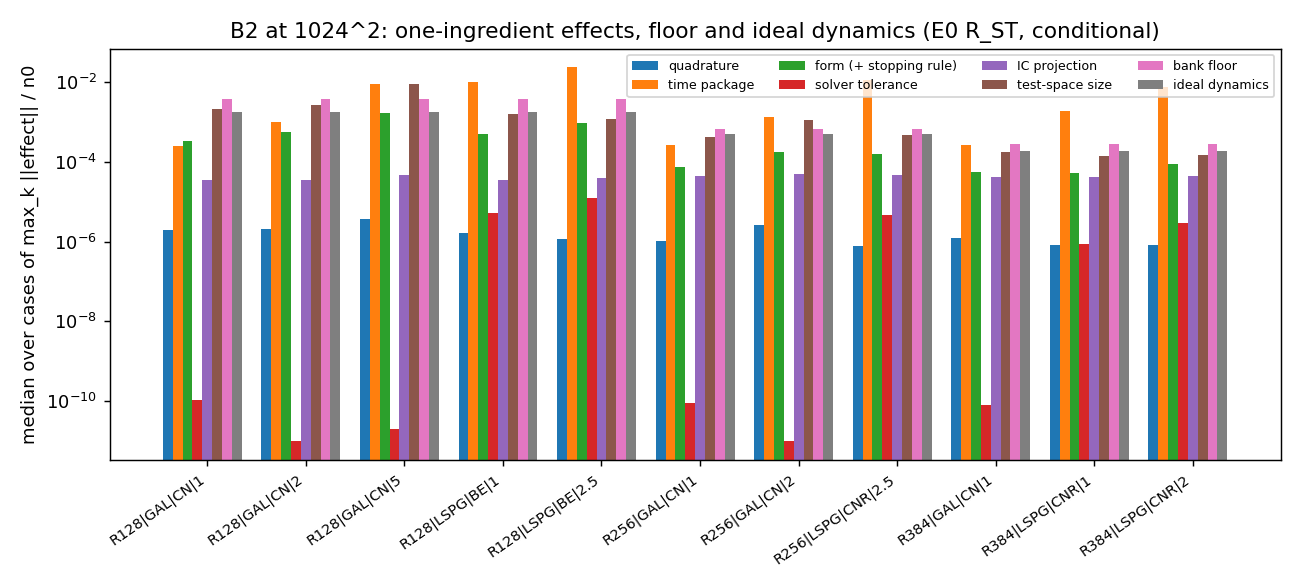
\includegraphics[width=0.48\linewidth]{figs/b_b2_1024.png}\hfill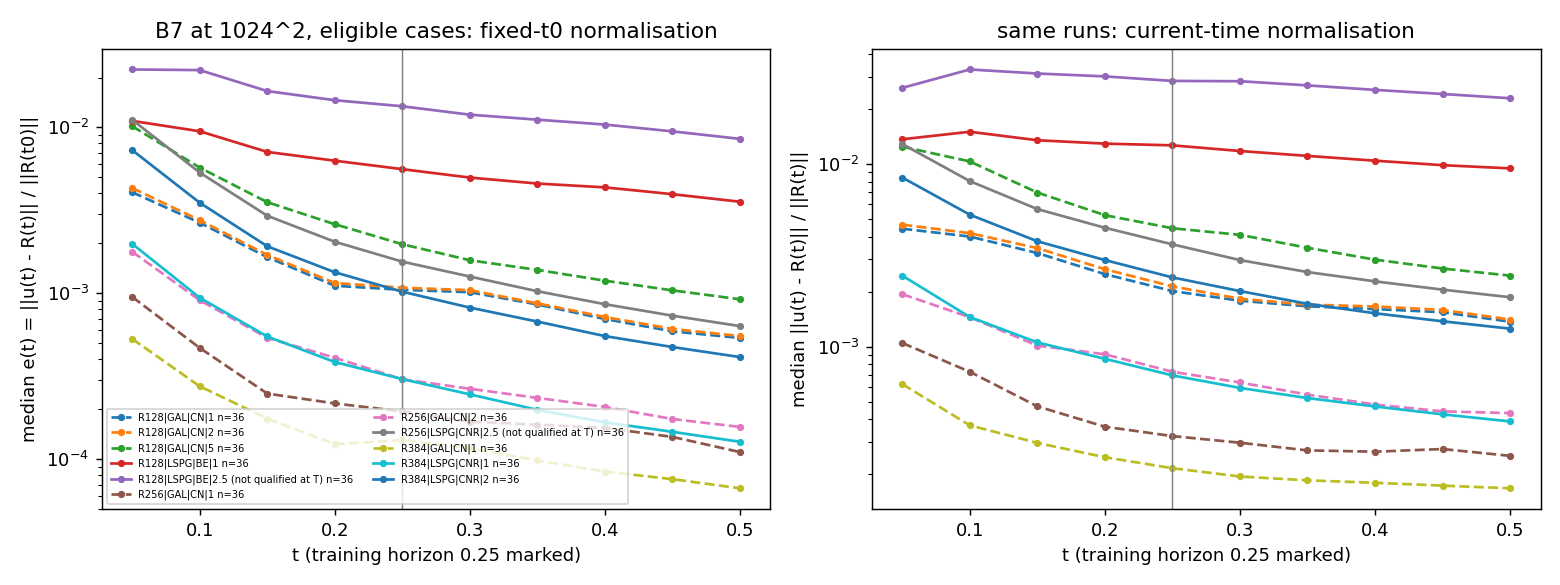
\includegraphics[width=0.48\linewidth]{figs/b_b7_1024.png}\end{center}
\subsection*{Corrections}
\retracted{Costs of E0's tight re-solve forced reruns without it (those cases non-rankable, A9). A later claim that disabling a tight retry cost rankable cases was itself corrected (A14.2: it cost none). A dominance tie rule compared only the top two candidates (A14.3; two counts changed, no label). A 3D reference mismatch traced to a last-bit inconsistency inside E0's store (A13).}
